% Options for packages loaded elsewhere
\PassOptionsToPackage{unicode}{hyperref}
\PassOptionsToPackage{hyphens}{url}
%
\documentclass[
  12pt,
  ignorenonframetext,
  aspectratio=169,
]{beamer}
\usepackage{pgfpages}
\setbeamertemplate{caption}[numbered]
\setbeamertemplate{caption label separator}{: }
\setbeamercolor{caption name}{fg=normal text.fg}
\beamertemplatenavigationsymbolsempty
% Prevent slide breaks in the middle of a paragraph
\widowpenalties 1 10000
\raggedbottom
\setbeamertemplate{part page}{
  \centering
  \begin{beamercolorbox}[sep=16pt,center]{part title}
    \usebeamerfont{part title}\insertpart\par
  \end{beamercolorbox}
}
\setbeamertemplate{section page}{
  \centering
  \begin{beamercolorbox}[sep=12pt,center]{part title}
    \usebeamerfont{section title}\insertsection\par
  \end{beamercolorbox}
}
\setbeamertemplate{subsection page}{
  \centering
  \begin{beamercolorbox}[sep=8pt,center]{part title}
    \usebeamerfont{subsection title}\insertsubsection\par
  \end{beamercolorbox}
}
\AtBeginPart{
  \frame{\partpage}
}
\AtBeginSection{
  \ifbibliography
  \else
    \frame{\sectionpage}
  \fi
}
\AtBeginSubsection{
  \frame{\subsectionpage}
}

\usepackage{amsmath,amssymb}
\usepackage{iftex}
\ifPDFTeX
  \usepackage[T1]{fontenc}
  \usepackage[utf8]{inputenc}
  \usepackage{textcomp} % provide euro and other symbols
\else % if luatex or xetex
  \usepackage{unicode-math}
  \defaultfontfeatures{Scale=MatchLowercase}
  \defaultfontfeatures[\rmfamily]{Ligatures=TeX,Scale=1}
\fi
\usepackage{lmodern}
\usetheme[]{Rochester}
\usecolortheme{spruce}
\usefonttheme{professionalfonts}
\ifPDFTeX\else  
    % xetex/luatex font selection
\fi
% Use upquote if available, for straight quotes in verbatim environments
\IfFileExists{upquote.sty}{\usepackage{upquote}}{}
\IfFileExists{microtype.sty}{% use microtype if available
  \usepackage[]{microtype}
  \UseMicrotypeSet[protrusion]{basicmath} % disable protrusion for tt fonts
}{}
\makeatletter
\@ifundefined{KOMAClassName}{% if non-KOMA class
  \IfFileExists{parskip.sty}{%
    \usepackage{parskip}
  }{% else
    \setlength{\parindent}{0pt}
    \setlength{\parskip}{6pt plus 2pt minus 1pt}}
}{% if KOMA class
  \KOMAoptions{parskip=half}}
\makeatother
\usepackage{xcolor}
\newif\ifbibliography
\setlength{\emergencystretch}{3em} % prevent overfull lines
\setcounter{secnumdepth}{-\maxdimen} % remove section numbering


\providecommand{\tightlist}{%
  \setlength{\itemsep}{0pt}\setlength{\parskip}{0pt}}\usepackage{longtable,booktabs,array}
\usepackage{calc} % for calculating minipage widths
\usepackage{caption}
% Make caption package work with longtable
\makeatletter
\def\fnum@table{\tablename~\thetable}
\makeatother
\usepackage{graphicx}
\makeatletter
\def\maxwidth{\ifdim\Gin@nat@width>\linewidth\linewidth\else\Gin@nat@width\fi}
\def\maxheight{\ifdim\Gin@nat@height>\textheight\textheight\else\Gin@nat@height\fi}
\makeatother
% Scale images if necessary, so that they will not overflow the page
% margins by default, and it is still possible to overwrite the defaults
% using explicit options in \includegraphics[width, height, ...]{}
\setkeys{Gin}{width=\maxwidth,height=\maxheight,keepaspectratio}
% Set default figure placement to htbp
\makeatletter
\def\fps@figure{htbp}
\makeatother
\newlength{\cslhangindent}
\setlength{\cslhangindent}{1.5em}
\newlength{\csllabelwidth}
\setlength{\csllabelwidth}{3em}
\newlength{\cslentryspacingunit} % times entry-spacing
\setlength{\cslentryspacingunit}{\parskip}
\newenvironment{CSLReferences}[2] % #1 hanging-ident, #2 entry spacing
 {% don't indent paragraphs
  \setlength{\parindent}{0pt}
  % turn on hanging indent if param 1 is 1
  \ifodd #1
  \let\oldpar\par
  \def\par{\hangindent=\cslhangindent\oldpar}
  \fi
  % set entry spacing
  \setlength{\parskip}{#2\cslentryspacingunit}
 }%
 {}
\usepackage{calc}
\newcommand{\CSLBlock}[1]{#1\hfill\break}
\newcommand{\CSLLeftMargin}[1]{\parbox[t]{\csllabelwidth}{#1}}
\newcommand{\CSLRightInline}[1]{\parbox[t]{\linewidth - \csllabelwidth}{#1}\break}
\newcommand{\CSLIndent}[1]{\hspace{\cslhangindent}#1}

\usepackage{booktabs}
\usepackage{longtable}
\usepackage{array}
\usepackage{multirow}
\usepackage{wrapfig}
\usepackage{float}
\usepackage{colortbl}
\usepackage{pdflscape}
\usepackage{tabu}
\usepackage{threeparttable}
\usepackage{threeparttablex}
\usepackage[normalem]{ulem}
\usepackage{makecell}
\usepackage{xcolor}
\usepackage{graphicx}
\setbeamerfont{itemize/enumerate body}{size=\footnotesize}
\setbeamerfont{itemize/enumerate subbody}{size=\footnotesize}
\setbeamerfont{itemize/enumerate subsubbody}{size=\footnotesize}
\makeatletter
\makeatother
\makeatletter
\makeatother
\makeatletter
\@ifpackageloaded{caption}{}{\usepackage{caption}}
\AtBeginDocument{%
\ifdefined\contentsname
  \renewcommand*\contentsname{Table of contents}
\else
  \newcommand\contentsname{Table of contents}
\fi
\ifdefined\listfigurename
  \renewcommand*\listfigurename{List of Figures}
\else
  \newcommand\listfigurename{List of Figures}
\fi
\ifdefined\listtablename
  \renewcommand*\listtablename{List of Tables}
\else
  \newcommand\listtablename{List of Tables}
\fi
\ifdefined\figurename
  \renewcommand*\figurename{Figure}
\else
  \newcommand\figurename{Figure}
\fi
\ifdefined\tablename
  \renewcommand*\tablename{Table}
\else
  \newcommand\tablename{Table}
\fi
}
\@ifpackageloaded{float}{}{\usepackage{float}}
\floatstyle{ruled}
\@ifundefined{c@chapter}{\newfloat{codelisting}{h}{lop}}{\newfloat{codelisting}{h}{lop}[chapter]}
\floatname{codelisting}{Listing}
\newcommand*\listoflistings{\listof{codelisting}{List of Listings}}
\makeatother
\makeatletter
\@ifpackageloaded{caption}{}{\usepackage{caption}}
\@ifpackageloaded{subcaption}{}{\usepackage{subcaption}}
\makeatother
\makeatletter
\@ifpackageloaded{tcolorbox}{}{\usepackage[skins,breakable]{tcolorbox}}
\makeatother
\makeatletter
\@ifundefined{shadecolor}{\definecolor{shadecolor}{rgb}{.97, .97, .97}}
\makeatother
\makeatletter
\makeatother
\makeatletter
\makeatother
\ifLuaTeX
  \usepackage{selnolig}  % disable illegal ligatures
\fi
\IfFileExists{bookmark.sty}{\usepackage{bookmark}}{\usepackage{hyperref}}
\IfFileExists{xurl.sty}{\usepackage{xurl}}{} % add URL line breaks if available
\urlstyle{same} % disable monospaced font for URLs
\hypersetup{
  pdftitle={ERA 5 calibration to Elexon power},
  pdfauthor={S. Gomez\^{}1},
  hidelinks,
  pdfcreator={LaTeX via pandoc}}

\title{ERA 5 calibration to Elexon power}
\author{S. Gomez\(^1\)}
\date{2026-07-09}
\institute{\(^1\)School of Mathematics, University of Edinburgh}

\begin{document}
\frame{\titlepage}
\ifdefined\Shaded\renewenvironment{Shaded}{\begin{tcolorbox}[breakable, enhanced, frame hidden, borderline west={3pt}{0pt}{shadecolor}, boxrule=0pt, interior hidden, sharp corners]}{\end{tcolorbox}}\fi

\renewcommand*\contentsname{Table of contents}
\begin{frame}[allowframebreaks]
  \frametitle{Table of contents}
  \tableofcontents[hideallsubsections]
\end{frame}
\hypertarget{sec-intro}{%
\section{Overview}\label{sec-intro}}

\begin{frame}{Updates}
\protect\hypertarget{sec-updates}{}
\begin{block}{New}
\protect\hypertarget{new}{}
\begin{itemize}
  \item OOS assessment
  \item Low wind events distribution
\end{itemize}
\end{block}
\end{frame}

\hypertarget{model-validation-framework}{%
\section{Model validation framework}\label{model-validation-framework}}

\begin{frame}{Framework for OOS assessment}
\protect\hypertarget{framework-for-oos-assessment}{}
\begin{columns}[T]
\begin{column}{0.5\textwidth}
\begin{itemize}
\tightlist
\item
  Run models on a sample of days

  \begin{itemize}
  \tightlist
  \item
    80/20 WF split for training and testing
  \item
    Training with 3 days to predict the 4th
  \item
    Randomly chosen 15 days from 2025, 5 per regime
  \end{itemize}
\item
  Evaluate performance at WF level
\item
  Error under aggregation

  \begin{itemize}
  \tightlist
  \item
    GB level
  \item
    Onshore / offshore
  \end{itemize}
\end{itemize}
\end{column}

\begin{column}{0.5\textwidth}
\centering

\small Sampled days for performance assessment

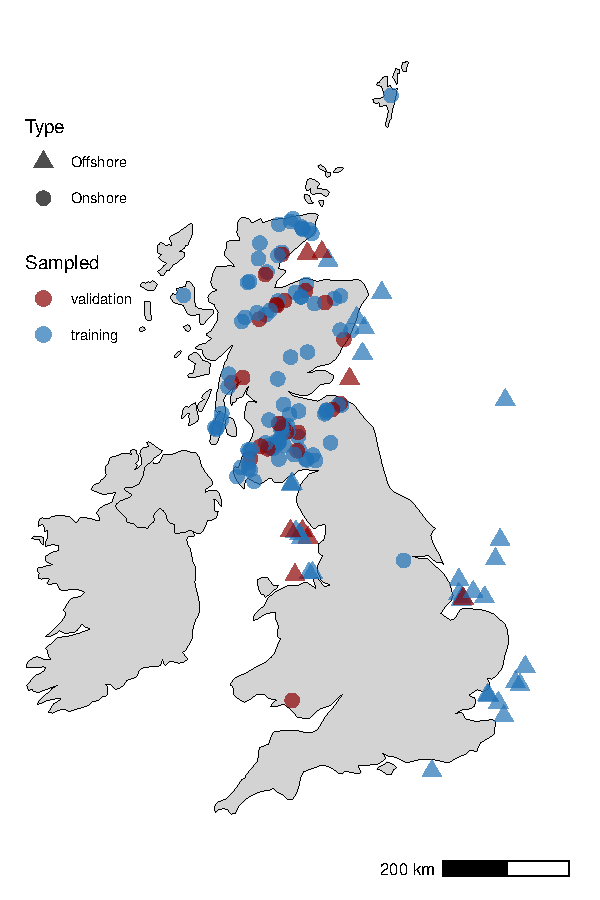
\includegraphics[width=\linewidth,height=6cm,keepaspectratio]{../fig/batch2025/trainsplit_wind_farm_locations_v0.pdf}
\end{column}
\end{columns}
\end{frame}

\begin{frame}{Sampled days in different regimes}
\protect\hypertarget{sampled-days-in-different-regimes}{}
\begin{columns}[T]
\begin{column}{0.5\textwidth}
\begin{itemize}
\tightlist
\item
  Objective is to assess performance by regime
\item
  OOS days are different regimes of wind speed
\item
  Previous 3 days can be anything
\end{itemize}
\end{column}

\begin{column}{0.5\textwidth}
\centering

\small Sampled days for performance assessment

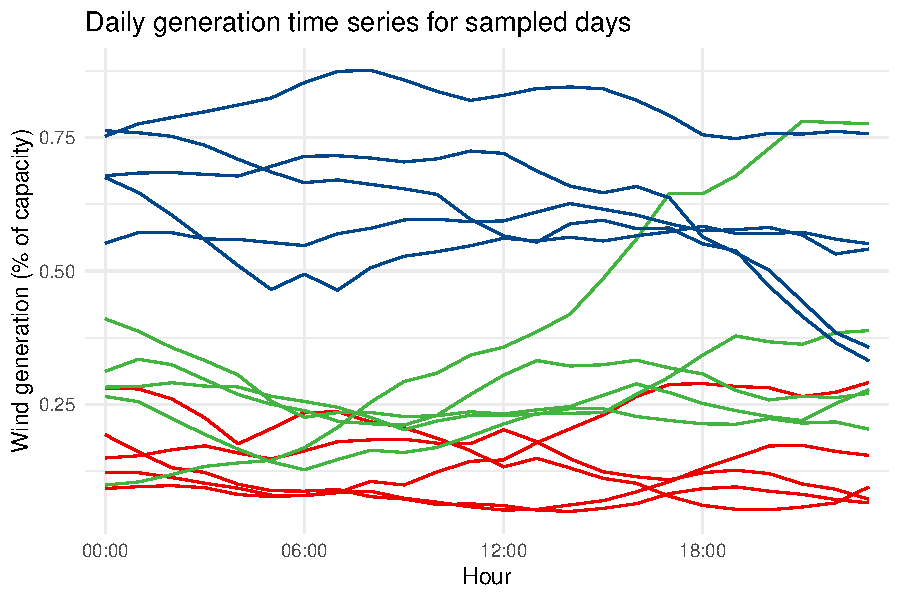
\includegraphics[width=\linewidth,height=5cm,keepaspectratio]{../fig/batch2025/daily_generation_time_series_sampled_days.pdf}
\end{column}
\end{columns}
\end{frame}

\begin{frame}{Model portfolio}
\protect\hypertarget{model-portfolio}{}
\begin{itemize}
\tightlist
\item
  Wind farm level models:

  \begin{itemize}
  \tightlist
  \item
    Generic Power Curve (ERA5 + generic PC estimate)
  \item
    Quantile Mapping
  \item
    Linear model
  \item
    AR1, AR2
  \item
    Spatiotemporal model fine mesh and coarser mesh
  \end{itemize}
\item
  Linear model at Great Britain (GB) level
\end{itemize}
\end{frame}

\hypertarget{out-of-sample-time}{%
\section{Out-of-sample time}\label{out-of-sample-time}}

\begin{frame}{Wind farm prediction bands}
\protect\hypertarget{wind-farm-prediction-bands}{}
\begin{columns}[T]
\begin{column}{0.5\textwidth}
\centering

\small Linear model

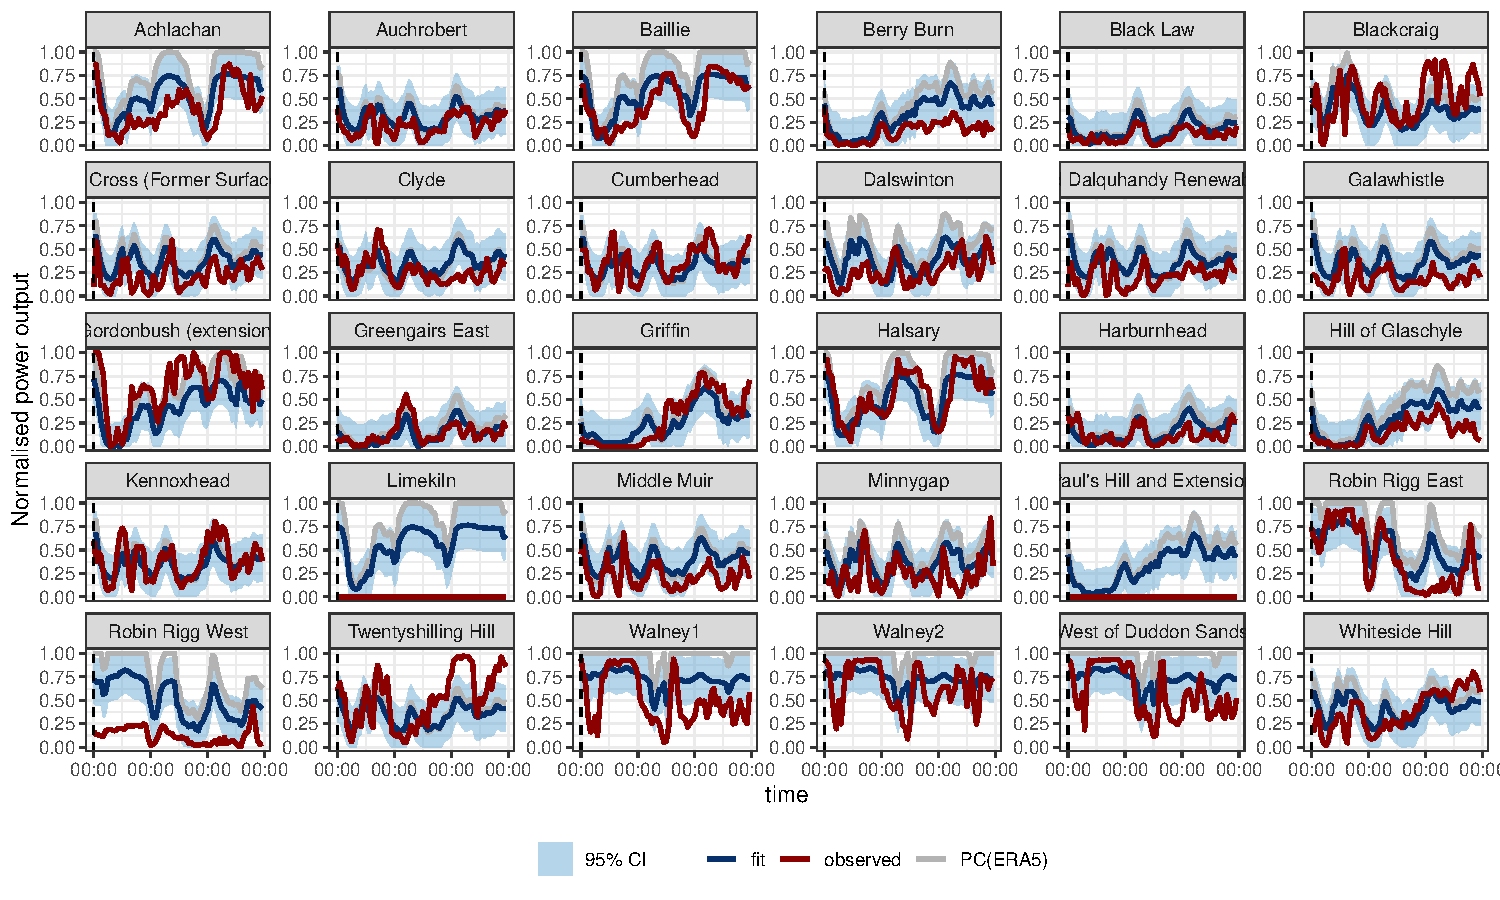
\includegraphics[width=\linewidth,height=5cm,keepaspectratio]{../fig/batch2025/WF_pred_band_lm_250127_2.pdf}
\end{column}

\begin{column}{0.5\textwidth}
\centering

\small Spatiotemporal model coarse

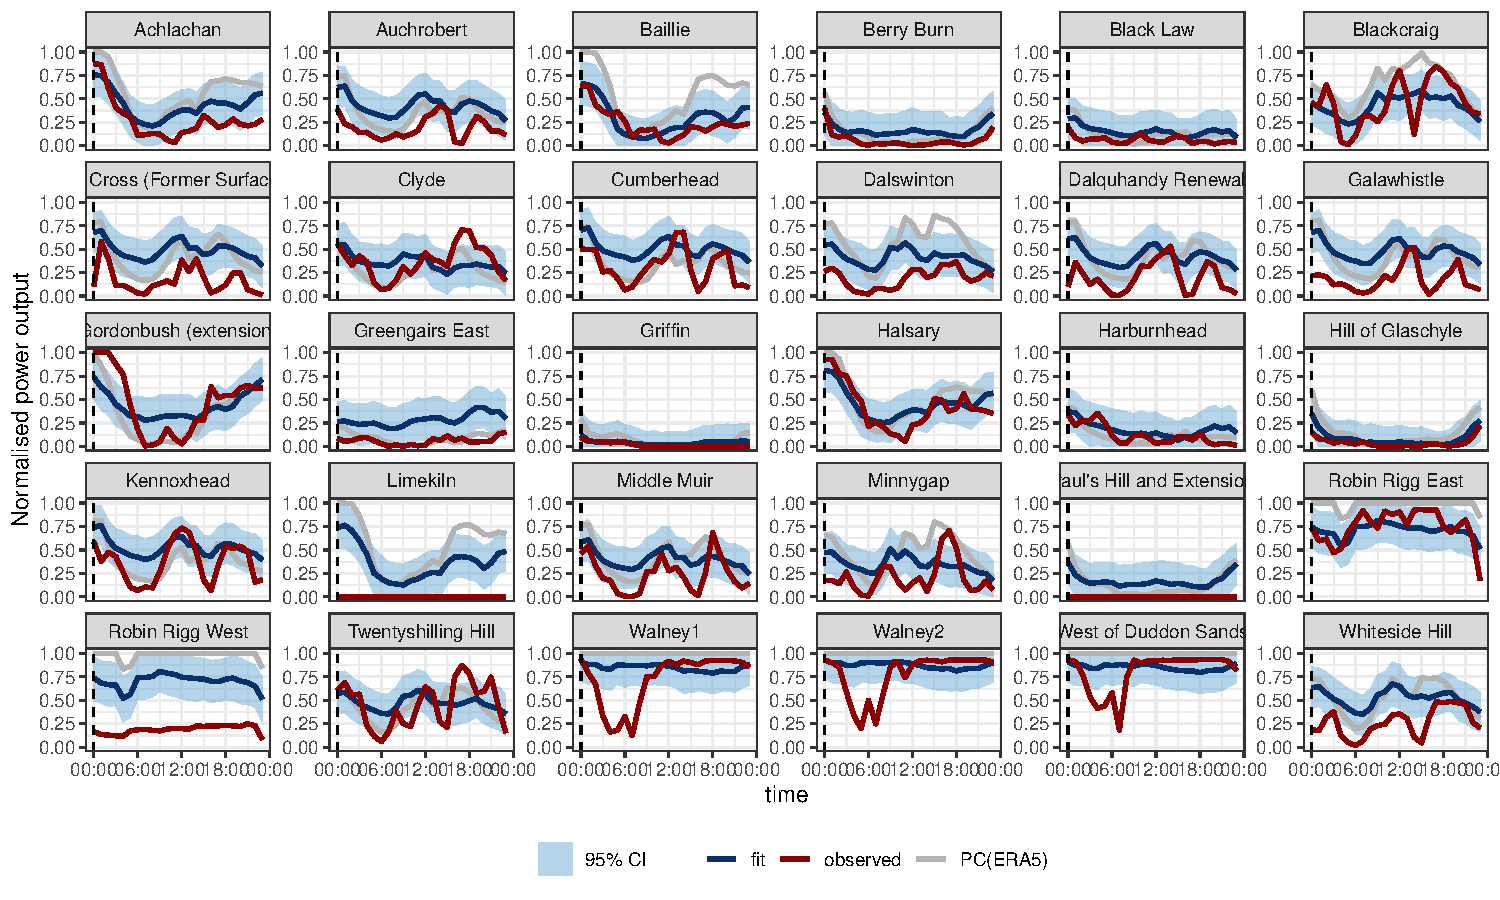
\includegraphics[width=\linewidth,height=5cm,keepaspectratio]{../fig/batch2025/WF_pred_band_st0_m1_250127_2.pdf}
\end{column}
\end{columns}
\end{frame}

\begin{frame}{Wind farm prediction bands}
\protect\hypertarget{wind-farm-prediction-bands-1}{}
\begin{columns}[T]
\begin{column}{0.5\textwidth}
\centering

\small 1D SPDE model

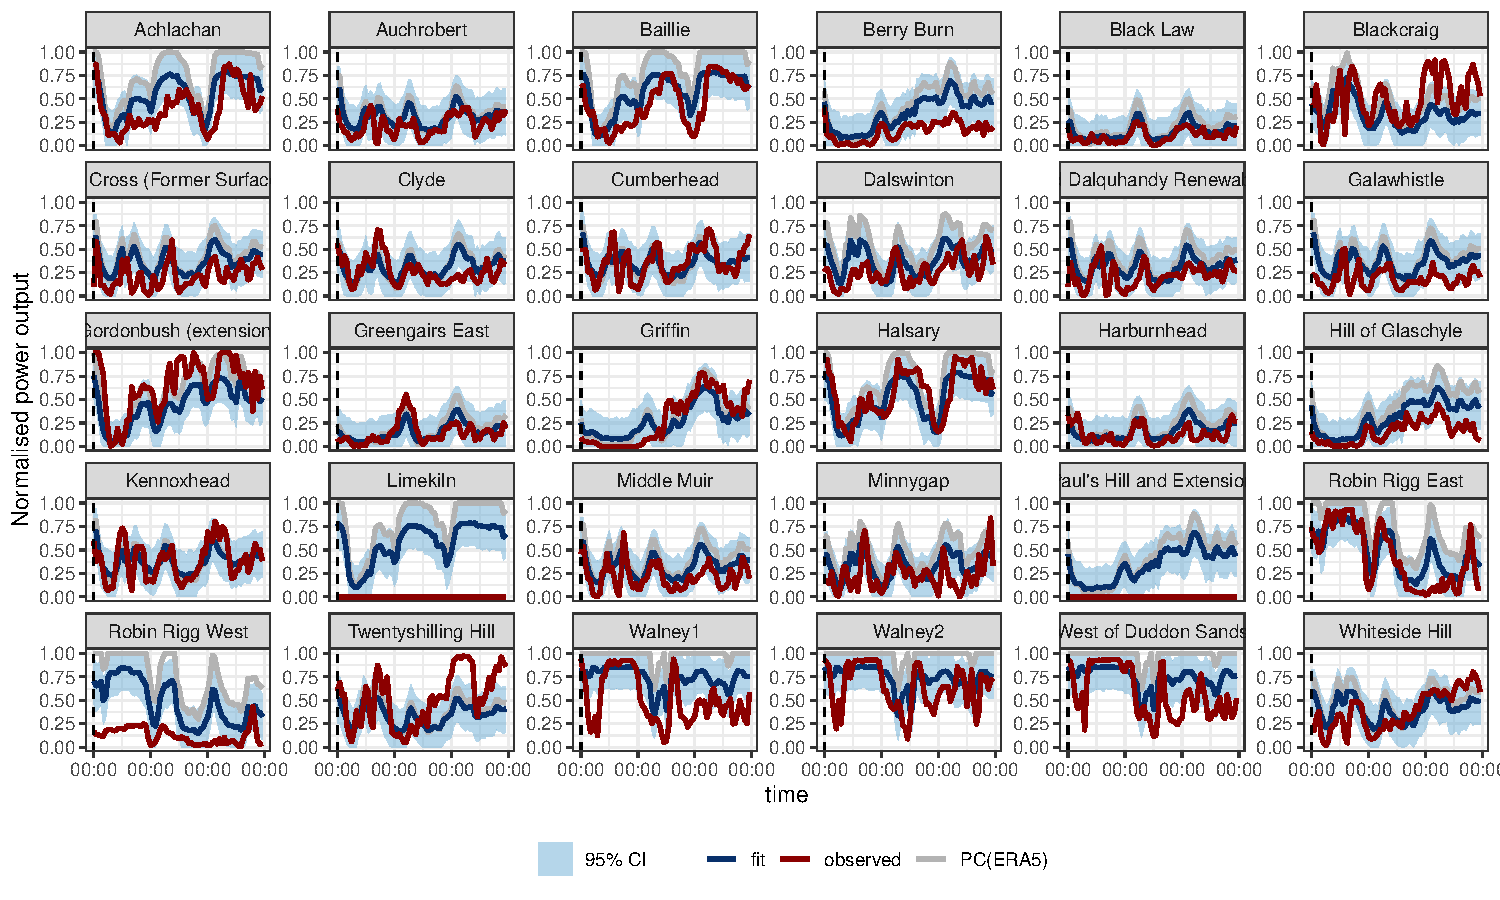
\includegraphics[width=\linewidth,height=5cm,keepaspectratio]{../fig/batch2025/WF_pred_band_spde1d_250127_2.pdf}
\end{column}

\begin{column}{0.5\textwidth}
\centering

\small AR1 model

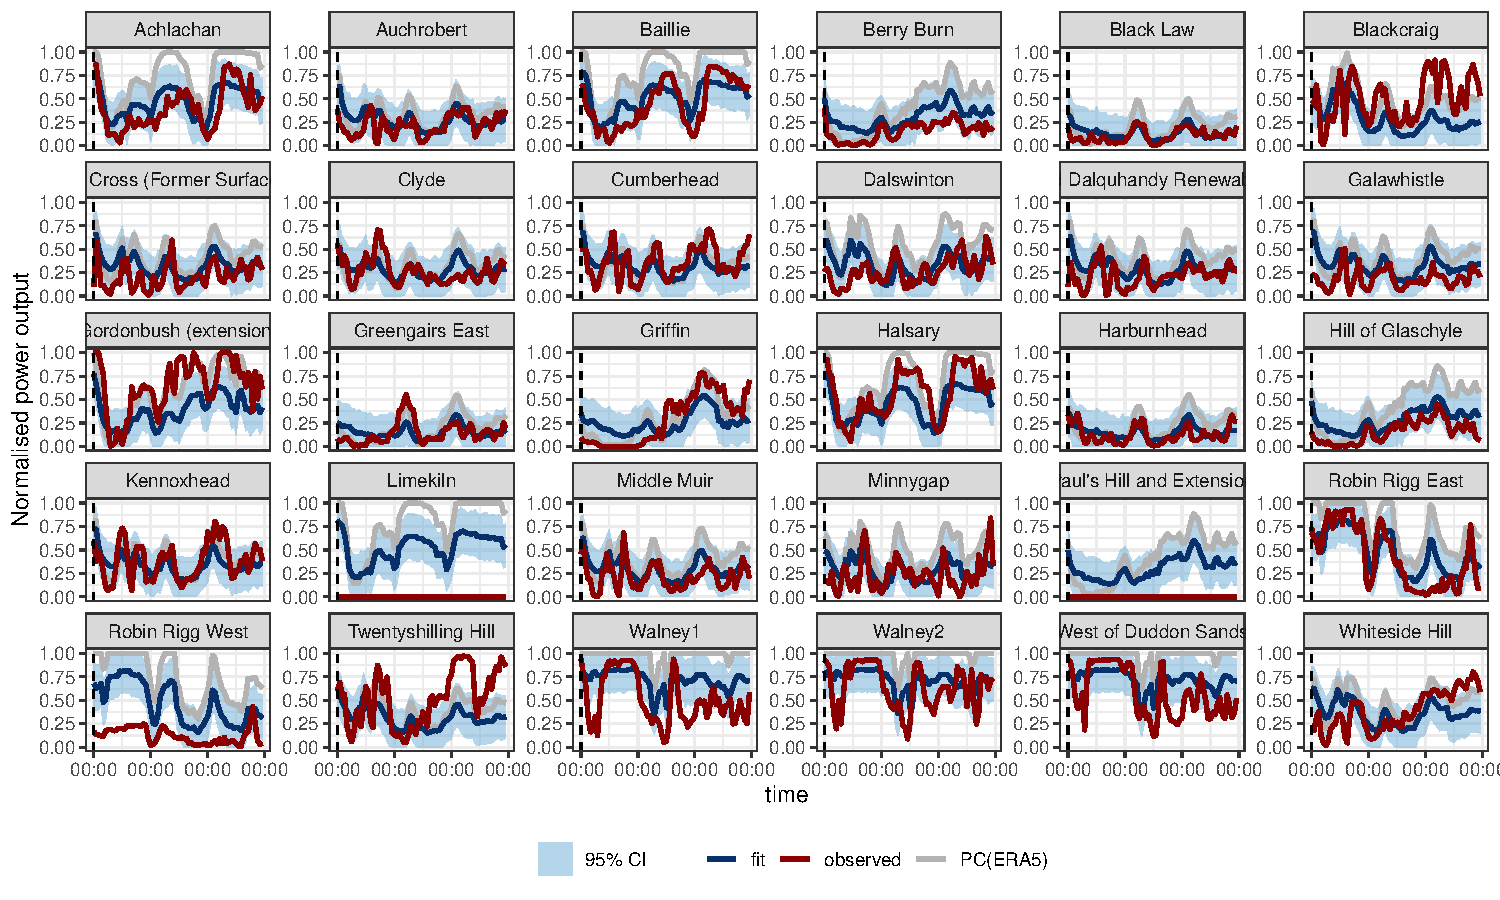
\includegraphics[width=\linewidth,height=5cm,keepaspectratio]{../fig/batch2025/WF_pred_band_ar1_250127_2.pdf}
\end{column}
\end{columns}
\end{frame}

\begin{frame}{Aggregated prediction bands}
\protect\hypertarget{aggregated-prediction-bands}{}
\begin{columns}[T]
\begin{column}{0.5\textwidth}
\centering

\small GB level

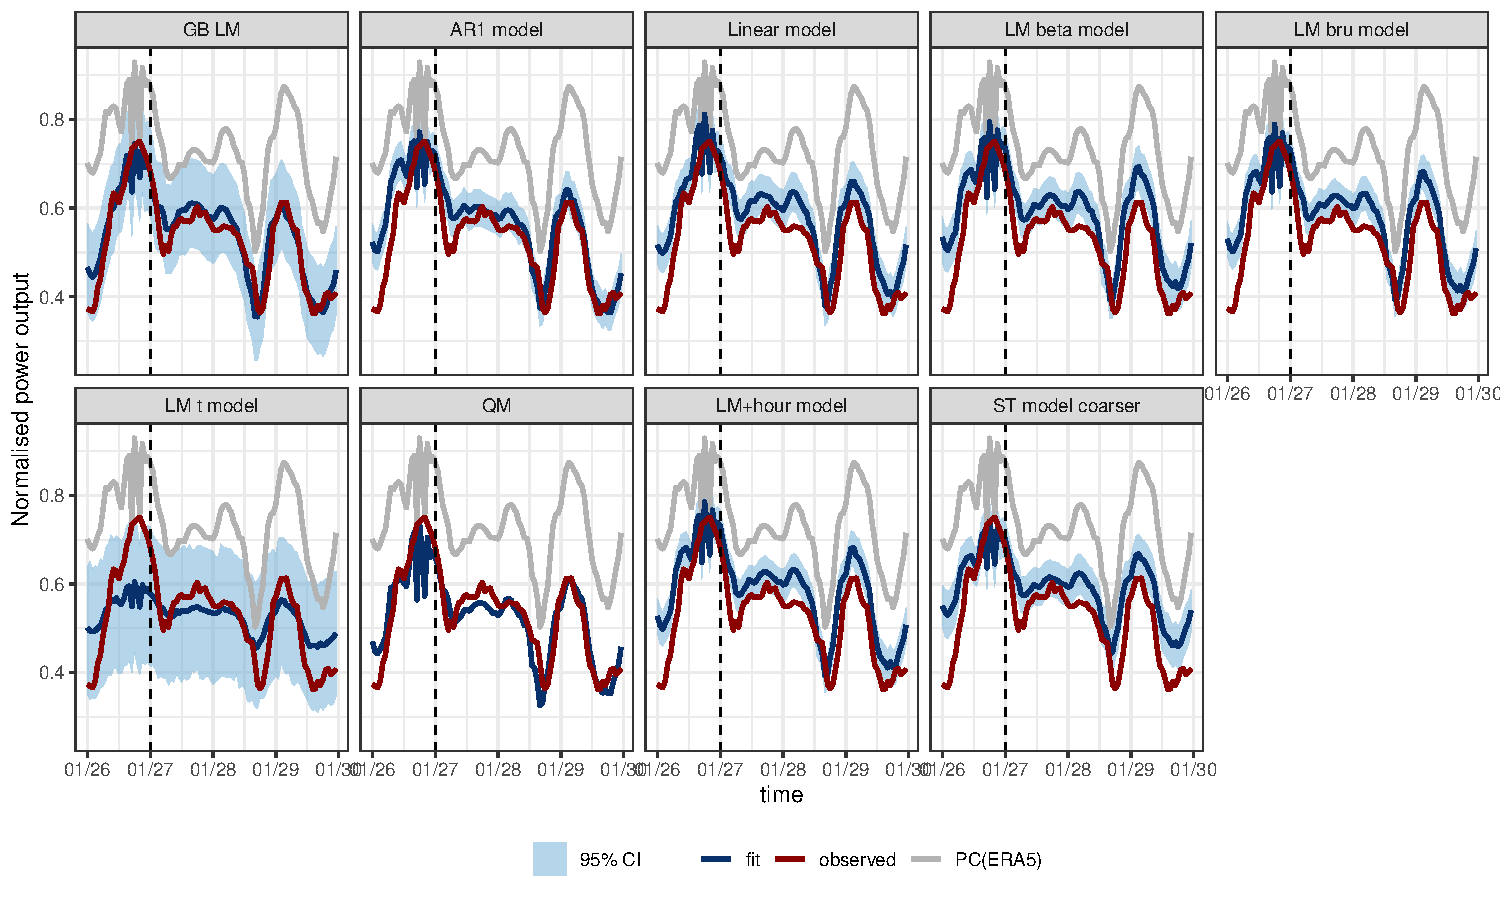
\includegraphics[width=\linewidth,height=5cm,keepaspectratio]{../fig/batch2025/GB_pred_band_250127.pdf}
\end{column}

\begin{column}{0.5\textwidth}
\end{column}
\end{columns}
\end{frame}

\begin{frame}{Day-ahead forecast coverage}
\protect\hypertarget{day-ahead-forecast-coverage}{}
\begin{columns}[T]
\begin{column}{0.5\textwidth}
\begin{itemize}
\tightlist
\item
  Models at WF can achieve target coverage
\item
  Aggregation reduces coverage
\item
  High regime more succeptible to coverage loss
\item
  Spatiotemporal model reduces coverage
\end{itemize}
\end{column}

\begin{column}{0.5\textwidth}
\centering

\small Coverage for day-ahead predictions

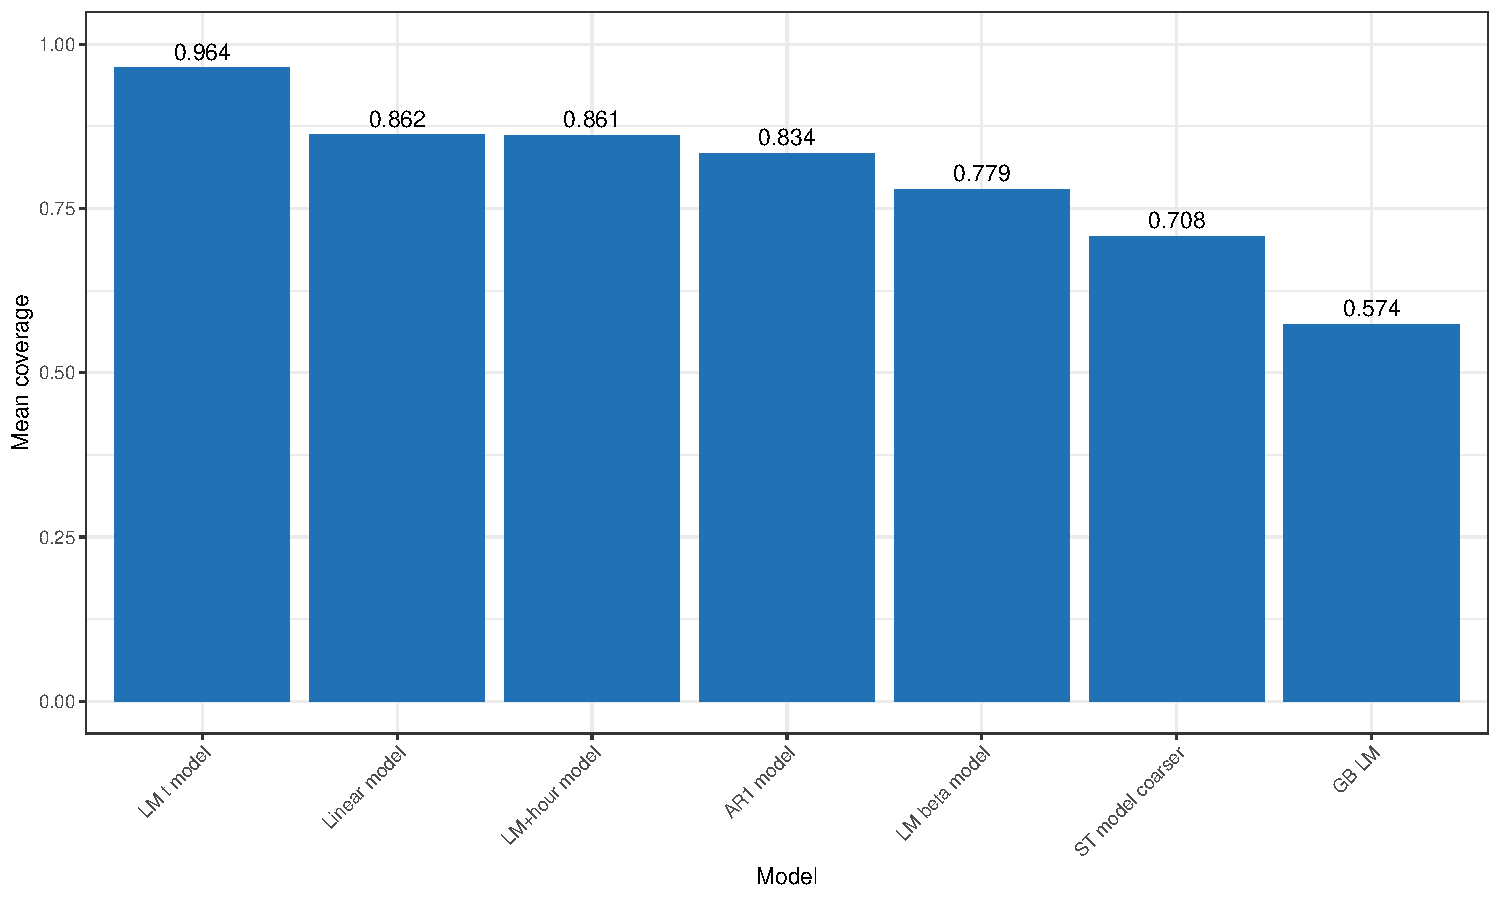
\includegraphics[width=\linewidth,height=5cm,keepaspectratio]{../fig/batch2025/WF_pred_band_coverage.pdf}
\end{column}
\end{columns}
\end{frame}

\begin{frame}{Coverage under aggregation}
\protect\hypertarget{coverage-under-aggregation}{}
\begin{columns}[T]
\begin{column}{0.5\textwidth}
\centering

\small GB level

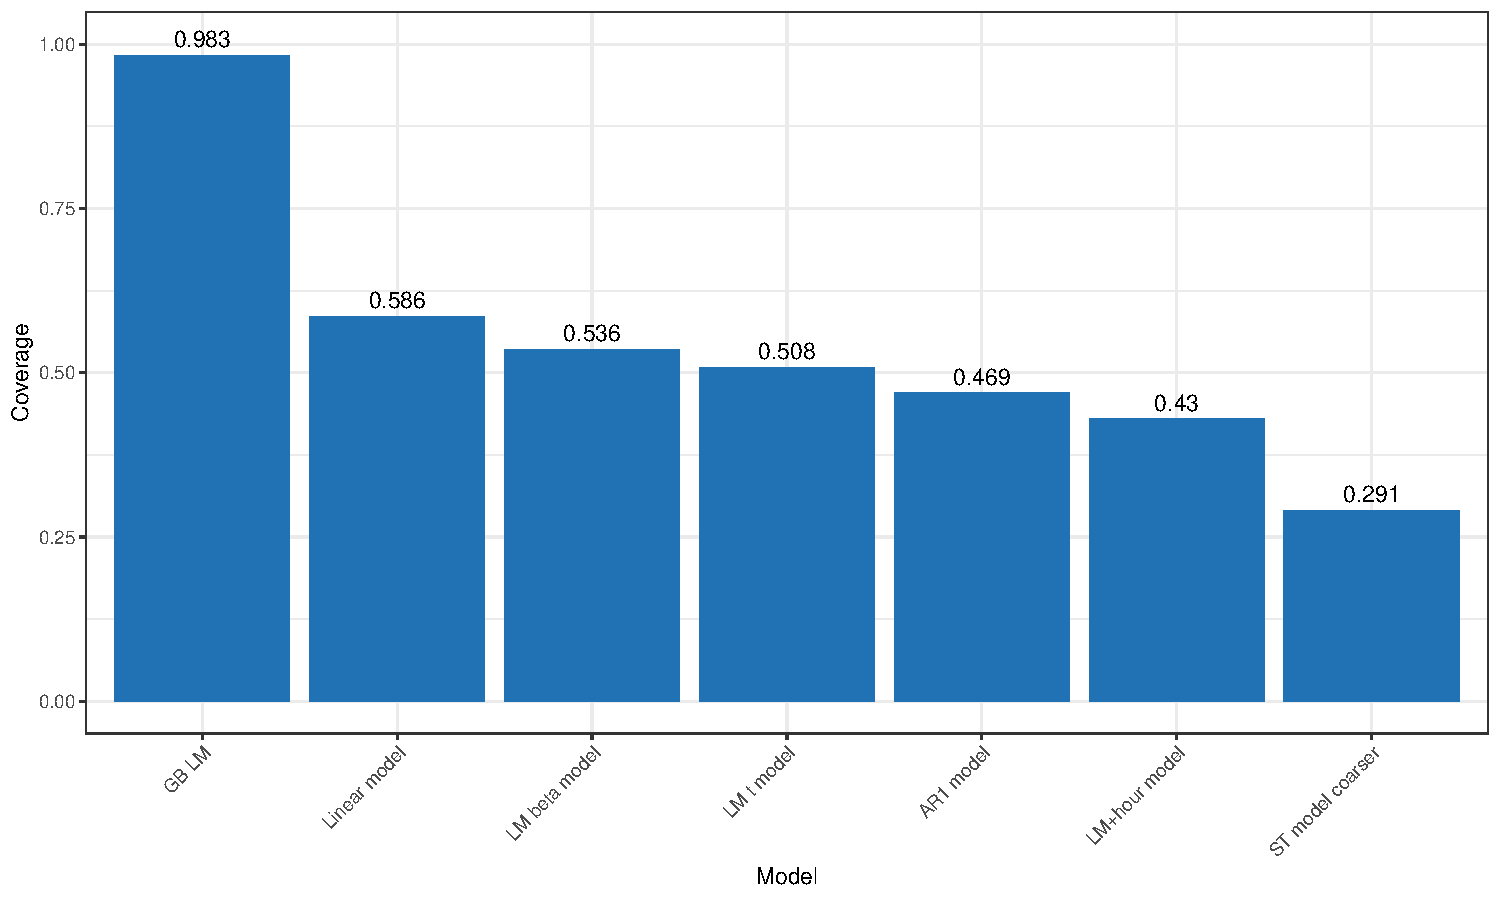
\includegraphics[width=\linewidth,height=5cm,keepaspectratio]{../fig/batch2025/GB_pred_band_coverage.pdf}
\end{column}

\begin{column}{0.5\textwidth}
\centering

\small Onshore / offshore

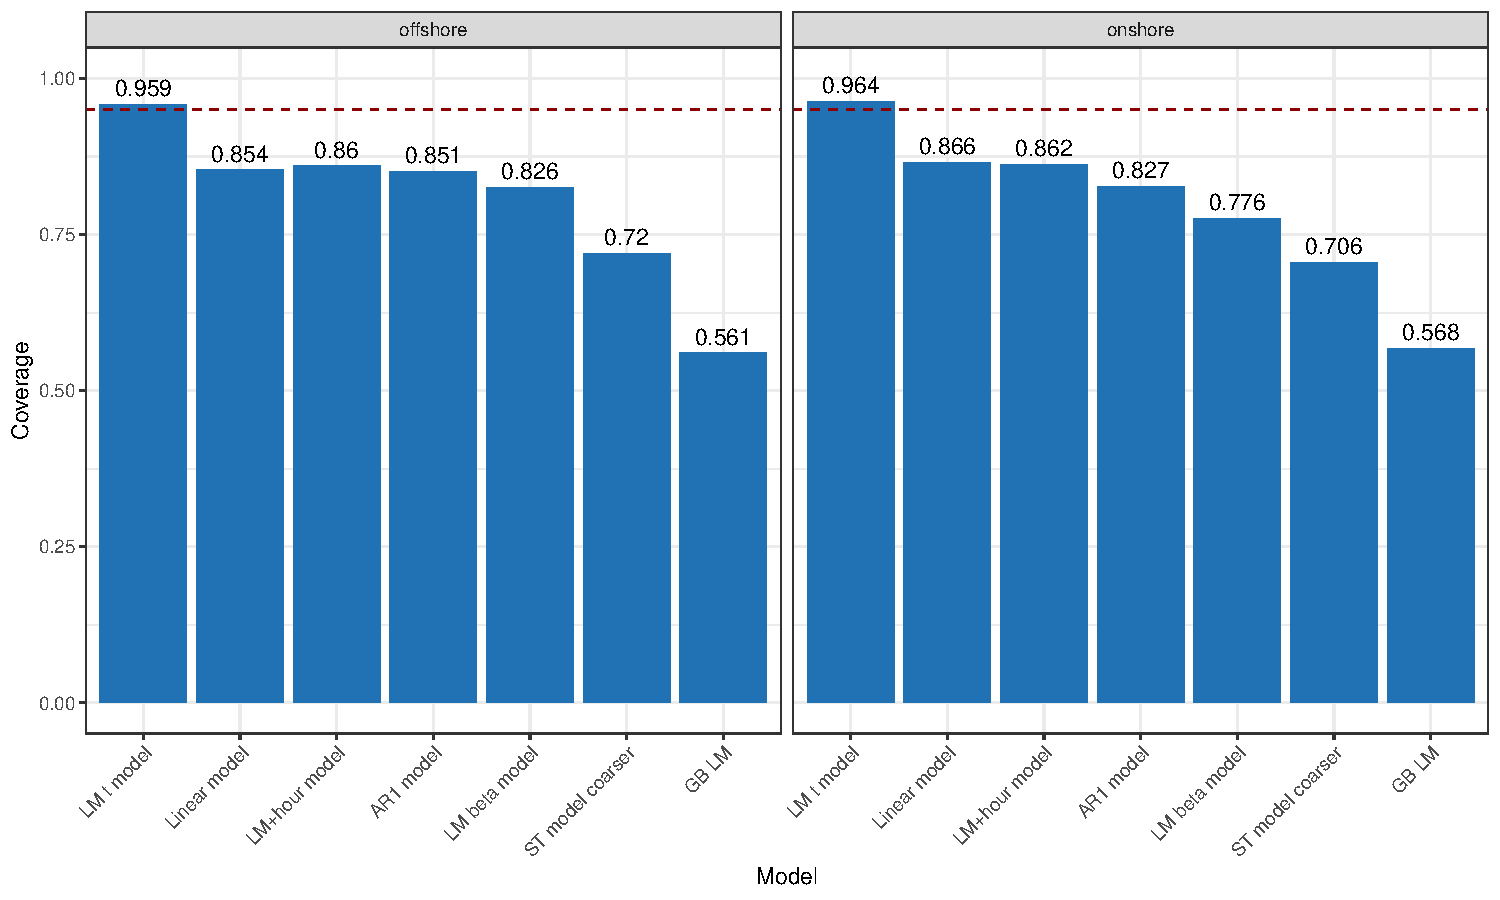
\includegraphics[width=\linewidth,height=5cm,keepaspectratio]{../fig/batch2025/GB_pred_band_coverage_tech.pdf}
\end{column}
\end{columns}
\end{frame}

\begin{frame}{Coverage under aggregation by regime}
\protect\hypertarget{coverage-under-aggregation-by-regime}{}
\centering

\small Regime aggregation

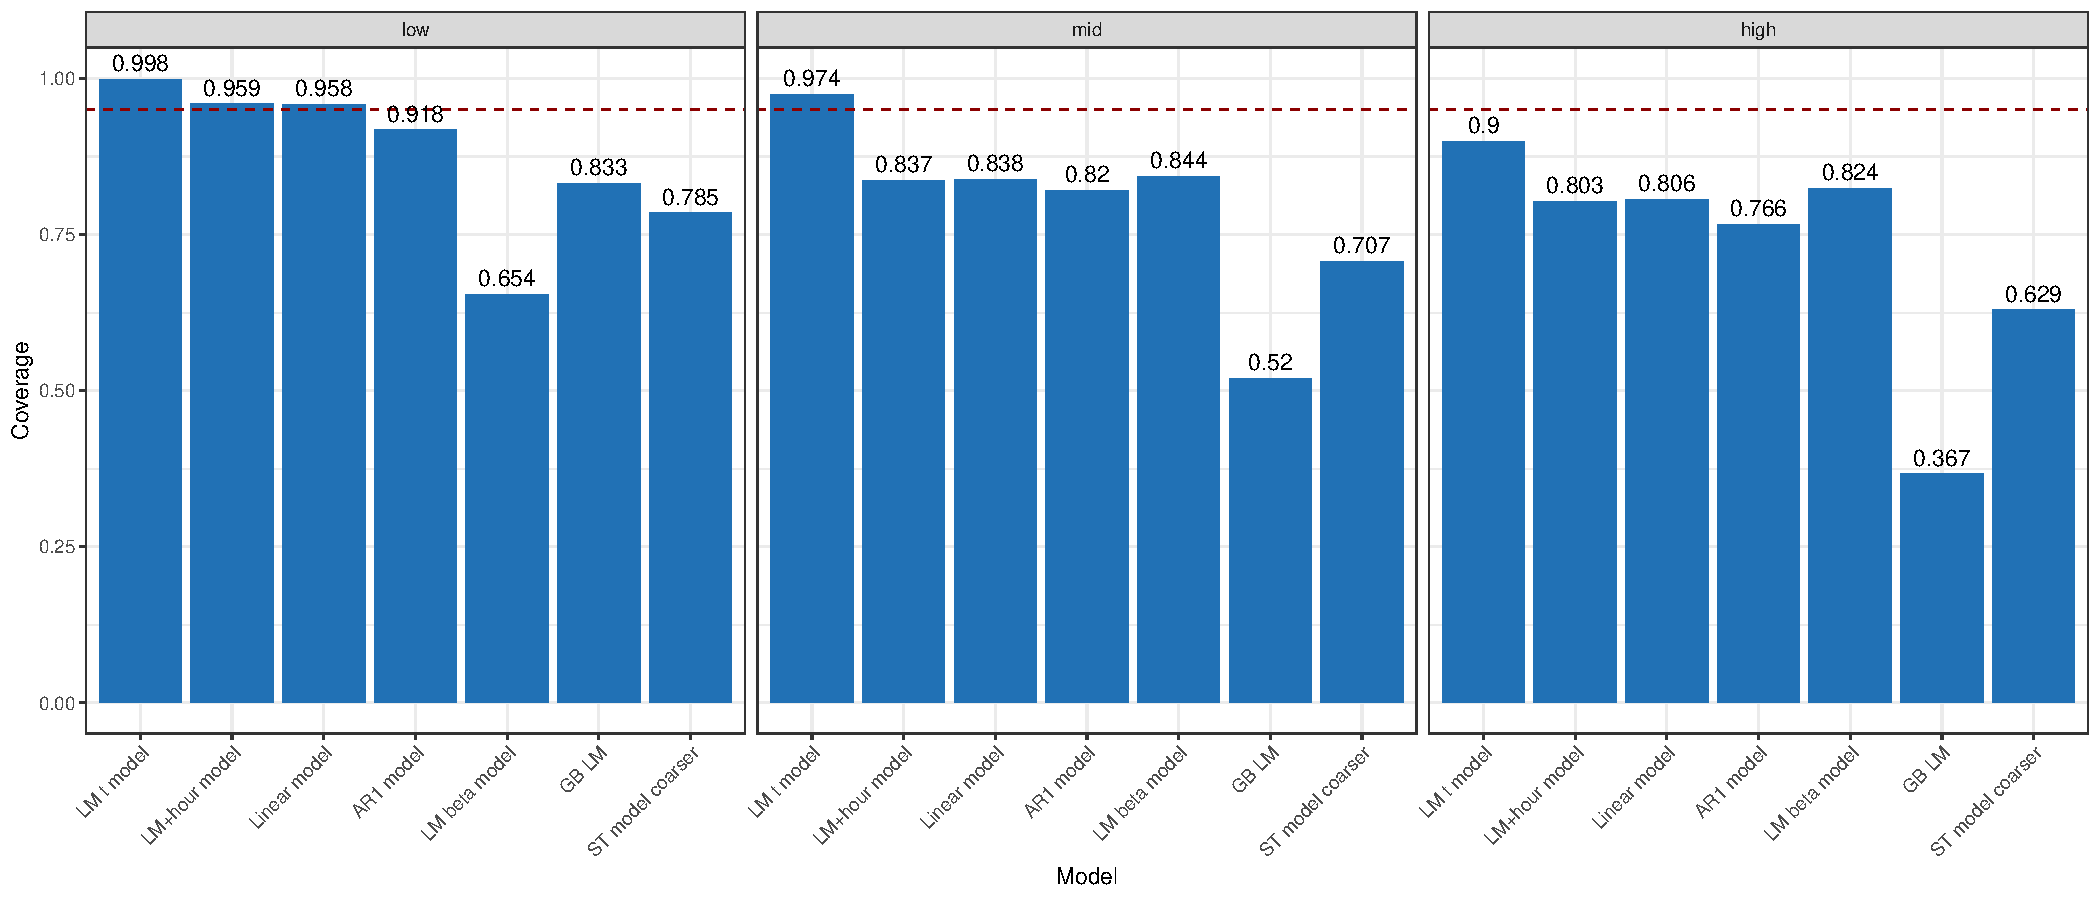
\includegraphics[width=\linewidth,height=5cm,keepaspectratio]{../fig/batch2025/GB_pred_band_coverage_regime.pdf}
\end{frame}

\hypertarget{out-of-sample-locations}{%
\section{Out-of-sample locations}\label{out-of-sample-locations}}

\begin{frame}{Wind farm prediction bands}
\protect\hypertarget{wind-farm-prediction-bands-2}{}
\begin{columns}[T]
\begin{column}{0.5\textwidth}
\centering

\small Linear model

\includegraphics[width=\linewidth,height=5cm,keepaspectratio]{../fig/batch2025/WF_pred_band_spaceoos_lm_250127_2.pdf}
\end{column}

\begin{column}{0.5\textwidth}
\centering

\small Spatiotemporal model coarse

\includegraphics[width=\linewidth,height=5cm,keepaspectratio]{../fig/batch2025/WF_pred_band_spaceoos_st0_m1_250127_2.pdf}
\end{column}
\end{columns}
\end{frame}

\begin{frame}{Wind farm prediction bands}
\protect\hypertarget{wind-farm-prediction-bands-3}{}
\begin{columns}[T]
\begin{column}{0.5\textwidth}
\centering

\small 1D SPDE model

\includegraphics[width=\linewidth,height=5cm,keepaspectratio]{../fig/batch2025/WF_pred_band_spaceoos_spde1d_250127_2.pdf}
\end{column}

\begin{column}{0.5\textwidth}
\centering

\small AR1 model

\includegraphics[width=\linewidth,height=5cm,keepaspectratio]{../fig/batch2025/WF_pred_band_spaceoos_ar1_250127_2.pdf}
\end{column}
\end{columns}
\end{frame}

\begin{frame}{Aggregated prediction bands}
\protect\hypertarget{aggregated-prediction-bands-1}{}
\begin{columns}[T]
\begin{column}{0.5\textwidth}
\centering

\small GB level

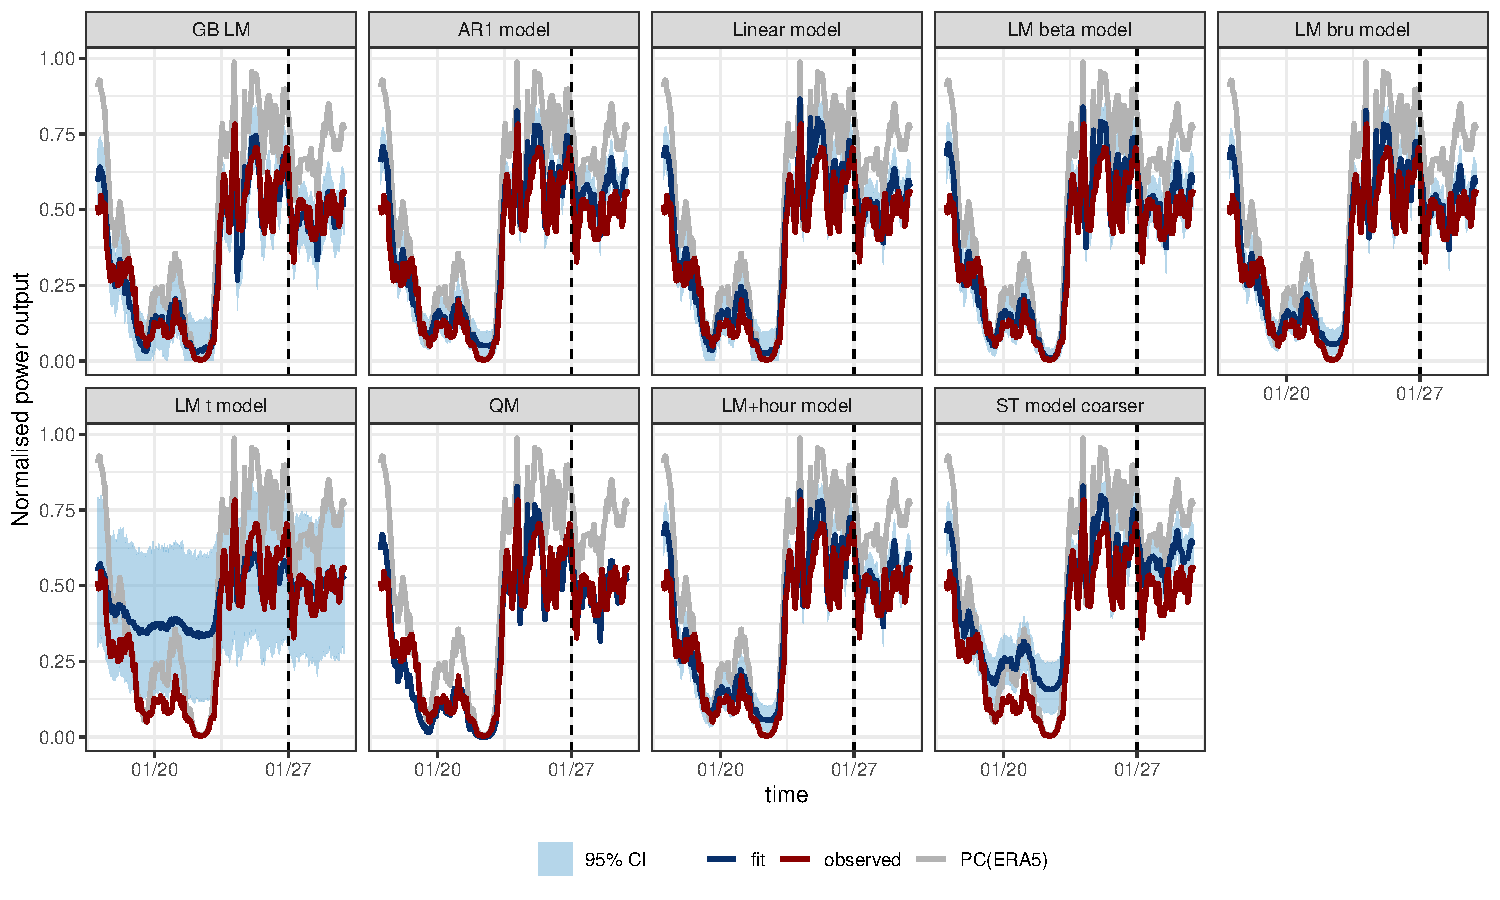
\includegraphics[width=\linewidth,height=5cm,keepaspectratio]{../fig/batch2025/GB_pred_band_spaceoos_250127.pdf}
\end{column}

\begin{column}{0.5\textwidth}
\end{column}
\end{columns}
\end{frame}

\begin{frame}{Day-ahead forecast coverage}
\protect\hypertarget{day-ahead-forecast-coverage-1}{}
\begin{columns}[T]
\begin{column}{0.5\textwidth}
\begin{itemize}
\tightlist
\item
  Models at WF can achieve target coverage
\item
  Aggregation reduces coverage
\item
  High regime more succeptible to coverage loss
\item
  Spatiotemporal model reduces coverage
\end{itemize}
\end{column}

\begin{column}{0.5\textwidth}
\centering

\small Coverage for day-ahead predictions

\includegraphics[width=\linewidth,height=5cm,keepaspectratio]{../fig/batch2025/WF_pred_band_spaceoos_coverage.pdf}
\end{column}
\end{columns}
\end{frame}

\begin{frame}{Coverage under aggregation}
\protect\hypertarget{coverage-under-aggregation-1}{}
\begin{columns}[T]
\begin{column}{0.5\textwidth}
\centering

\small GB level

\includegraphics[width=\linewidth,height=5cm,keepaspectratio]{../fig/batch2025/GB_pred_band_spaceoos_coverage.pdf}
\end{column}

\begin{column}{0.5\textwidth}
\centering

\small Onshore / offshore

\includegraphics[width=\linewidth,height=5cm,keepaspectratio]{../fig/batch2025/GB_pred_band_spaceoos_coverage_tech.pdf}
\end{column}
\end{columns}
\end{frame}

\begin{frame}{Coverage under aggregation by regime}
\protect\hypertarget{coverage-under-aggregation-by-regime-1}{}
\centering

\small Regime aggregation

\includegraphics[width=\linewidth,height=5cm,keepaspectratio]{../fig/batch2025/GB_pred_band_spaceoos_coverage_regime.pdf}

\begin{columns}[T]
\begin{column}{0.5\textwidth}
\begin{itemize}
\tightlist
\item
  Attaining coverage in unseen locations is more challenging
\item
  Isolated locations result in high uncertainty
\item
  Location specific events may affect coverage
\item
  Spatiotemporal model reduces coverage
\end{itemize}
\end{column}

\begin{column}{0.5\textwidth}
\centering

\small Coverage for day-ahead predictions

\includegraphics[width=\linewidth,height=5cm,keepaspectratio]{../fig/batch2025/WF_pred_band_spaceoos_coverage.pdf}
\end{column}
\end{columns}
\end{frame}

\begin{frame}{Meshes for spatiotemporal models}
\protect\hypertarget{meshes-for-spatiotemporal-models}{}
\begin{columns}[T]
\begin{column}{0.5\textwidth}
\centering

Coarse mesh


\includegraphics[width=\linewidth,height=6cm,keepaspectratio]{/home/s2441782/Documents/elexon/extra/mesh_figs/spatial_mesh_coarse_250121.pdf}
\end{column}

\begin{column}{0.5\textwidth}
\centering

Fine mesh


\includegraphics[width=\linewidth,height=6cm,keepaspectratio]{/home/s2441782/Documents/elexon/extra/mesh_figs/spatial_mesh_fine_250121.pdf}
\end{column}
\end{columns}
\end{frame}

\hypertarget{error-metrics-and-performance-assessment}{%
\section*{Error metrics and performance
assessment}\label{error-metrics-and-performance-assessment}}
\addcontentsline{toc}{section}{Error metrics and performance assessment}

\begin{frame}{Error metrics}
\protect\hypertarget{error-metrics}{}
\begin{table}
\centering
\resizebox{\ifdim\width>\linewidth\linewidth\else\width\fi}{!}{
\begin{tabular}{l|r|r|l}
\hline
model & RMSE & MAE & Bias\\
\hline
QM & 0.210 & 0.135 & 1.58e-04\\
\hline
GB LM & 0.191 & 0.130 & 2.12e-02\\
\hline
Linear model & 0.168 & 0.117 & 1.76e-03\\
\hline
1D SPDE model & 0.167 & 0.116 & 1.46e-03\\
\hline
AR2 model & 0.164 & 0.113 & 1.45e-03\\
\hline
AR1 model & 0.164 & 0.113 & 1.44e-03\\
\hline
Spatio-temporal coarse & 0.124 & 0.082 & 1.26e-03\\
\hline
Spatio-temporal fine & 0.097 & 0.061 & 1.16e-03\\
\hline
\end{tabular}}
\end{table}
\end{frame}

\begin{frame}{Error metrics by regime}
\protect\hypertarget{error-metrics-by-regime}{}
\vspace{-0.5cm}

\begin{table}
\centering
\resizebox{\ifdim\width>\linewidth\linewidth\else\width\fi}{!}{
\begin{tabular}[t]{lccccccccc}
\toprule
\multicolumn{1}{c}{ } & \multicolumn{3}{c}{Low} & \multicolumn{3}{c}{Mid} & \multicolumn{3}{c}{High} \\
\cmidrule(l{3pt}r{3pt}){2-4} \cmidrule(l{3pt}r{3pt}){5-7} \cmidrule(l{3pt}r{3pt}){8-10}
Model & RMSE & Bias & MAE & RMSE & Bias & MAE & RMSE & Bias & MAE\\
\midrule
QM & 0.110 & 0.062 & -1.59e-03 & 0.196 & 0.133 & 1.08e-04 & 0.305 & 0.219 & 2.21e-03\\
GB LM & 0.108 & 0.069 & 2.05e-02 & 0.186 & 0.132 & 2.44e-02 & 0.262 & 0.193 & 1.44e-02\\
1D SPDE model & 0.093 & 0.059 & 7.34e-03 & 0.160 & 0.115 & 2.50e-03 & 0.234 & 0.179 & -7.56e-03\\
Linear model & 0.092 & 0.059 & 6.57e-03 & 0.162 & 0.117 & 2.26e-03 & 0.235 & 0.183 & -4.75e-03\\
AR2 model & 0.089 & 0.056 & 3.07e-03 & 0.156 & 0.112 & 1.24e-03 & 0.230 & 0.176 & 1.49e-04\\
\addlinespace
AR1 model & 0.089 & 0.056 & 3.05e-03 & 0.156 & 0.112 & 1.22e-03 & 0.230 & 0.176 & 1.85e-04\\
Spatio-temporal coarse & 0.061 & 0.037 & 2.22e-03 & 0.117 & 0.081 & 1.13e-03 & 0.180 & 0.132 & 5.07e-04\\
Spatio-temporal fine & 0.048 & 0.028 & 1.75e-03 & 0.088 & 0.059 & 1.05e-03 & 0.145 & 0.101 & 7.84e-04\\
\bottomrule
\end{tabular}}
\end{table}
\end{frame}

\begin{frame}{Error metrics by technology}
\protect\hypertarget{error-metrics-by-technology}{}
\vspace{-0.5cm}

\begin{table}
\centering
\resizebox{\ifdim\width>\linewidth\linewidth\else\width\fi}{!}{
\begin{tabular}[t]{lcccccc}
\toprule
\multicolumn{1}{c}{ } & \multicolumn{3}{c}{Offshore} & \multicolumn{3}{c}{Onshore} \\
\cmidrule(l{3pt}r{3pt}){2-4} \cmidrule(l{3pt}r{3pt}){5-7}
Model & RMSE & Bias & MAE & RMSE & Bias & MAE\\
\midrule
QM & 0.213 & 0.139 & 5.85e-02 & 0.209 & 0.133 & -1.85e-02\\
GB LM & 0.184 & 0.127 & 8.26e-03 & 0.193 & 0.131 & 2.54e-02\\
1D SPDE model & 0.172 & 0.119 & 6.88e-04 & 0.166 & 0.114 & 1.70e-03\\
AR1 model & 0.169 & 0.117 & 6.72e-04 & 0.162 & 0.111 & 1.68e-03\\
AR2 model & 0.169 & 0.117 & 7.36e-04 & 0.162 & 0.111 & 1.67e-03\\
\addlinespace
Linear model & 0.157 & 0.113 & 2.84e-03 & 0.172 & 0.118 & 1.42e-03\\
Spatio-temporal coarse & 0.098 & 0.066 & 1.26e-03 & 0.131 & 0.087 & 1.26e-03\\
Spatio-temporal fine & 0.073 & 0.048 & 5.82e-04 & 0.103 & 0.065 & 1.34e-03\\
\bottomrule
\end{tabular}}
\end{table}
\end{frame}

\begin{frame}{Low wind speed events}
\protect\hypertarget{low-wind-speed-events}{}
\centering

Low wind speed events distribution
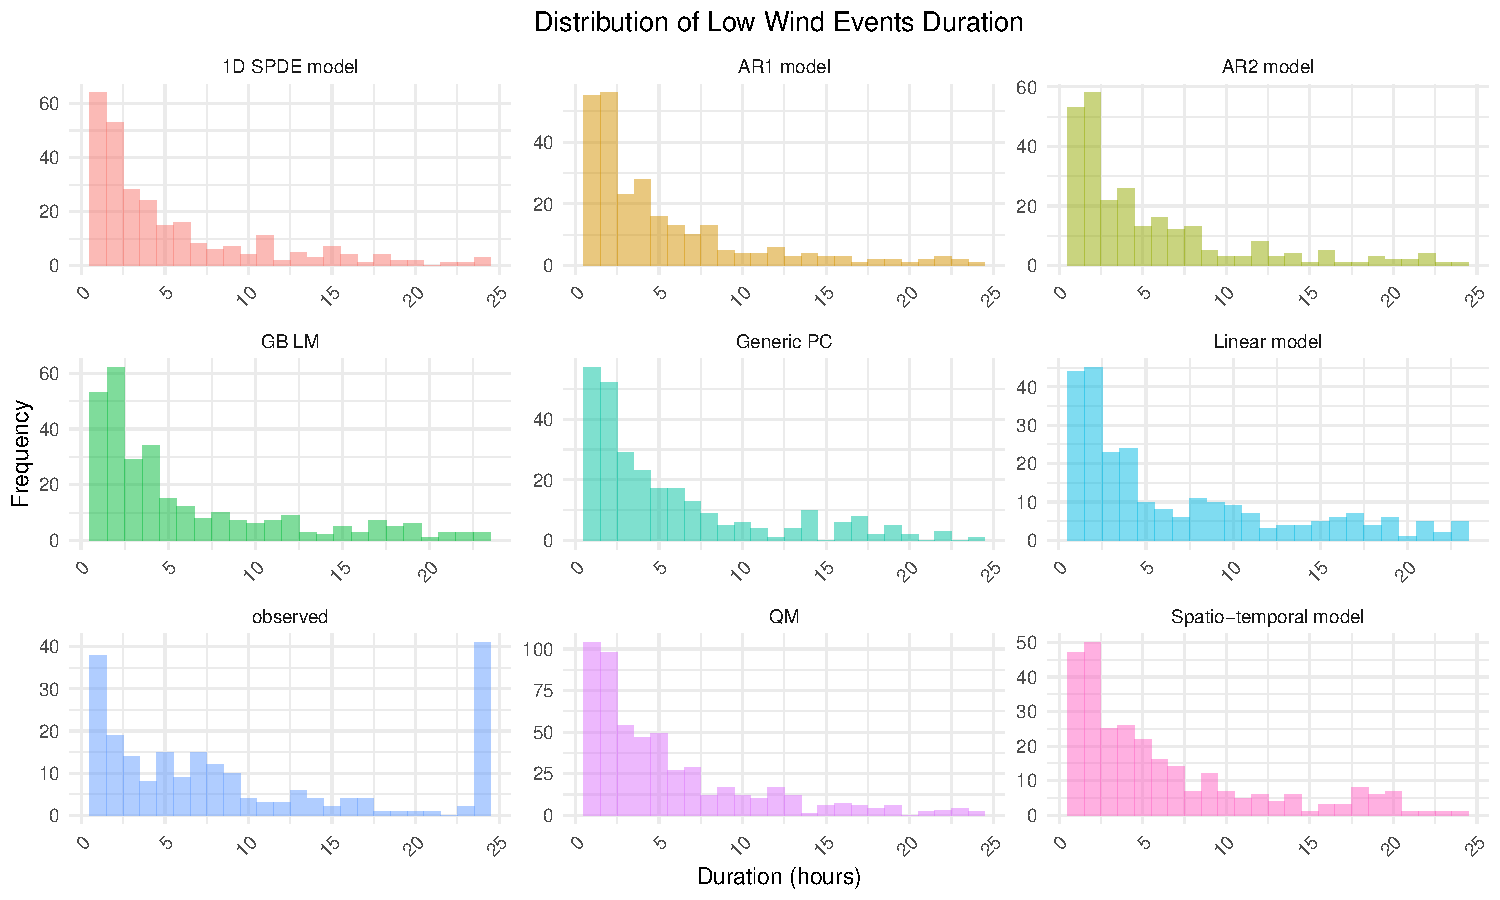
\includegraphics[width=\linewidth,height=5cm,keepaspectratio]{../fig/batch3days/low_wind_duration_dist.pdf}
\end{frame}

\hypertarget{spatiotemporal-calibration-model}{%
\section*{Spatiotemporal calibration
model}\label{spatiotemporal-calibration-model}}
\addcontentsline{toc}{section}{Spatiotemporal calibration model}

\begin{frame}{Model overview}
\protect\hypertarget{model-overview}{}
\begin{equation}
    \mathbb{E}(p^{\mathrm{calib}}_{it})
    = \alpha + \beta_{k} + \beta_m + \beta_h
    + s_p(\hat{p}_{it}) + s_w(w_{it})
    + u_{it},
    \label{eq:bayes_spat}
  \end{equation}

\begin{itemize}
\tightlist
\item
  Calibrated power: corrected output at site \emph{i}, time \emph{t}.\\
\item
  \(\alpha\): intercept.\\
\item
  Fixed effects \(\beta_k, \beta_m, \beta_h\): location/season/time
  structure.
\item
  ERA5 correction \(s_p\): bias adjustment of ERA5 + generic PC
  estimate.\\
\item
  Wind effect \(s_w\): nonlinear wind--power correction.\\
\item
  Spatiotemporal effect \(u_{it}\): Spatial component + AR1 error.
\end{itemize}
\end{frame}

\begin{frame}{References}
\protect\hypertarget{references}{}
\hypertarget{refs}{}
\begin{CSLReferences}{1}{0}
\leavevmode\vadjust pre{\hypertarget{ref-cannon_using_2015}{}}%
Cannon, D. J., D. J. Brayshaw, J. Methven, P. J. Coker, and D. Lenaghan.
2015. {``Using Reanalysis Data to Quantify Extreme Wind Power Generation
Statistics: A 33 Year Case Study in Great Britain.''} \emph{Renewable
Energy} 75 (March): 767--78. \url{https://centaur.reading.ac.uk/38448/}.

\leavevmode\vadjust pre{\hypertarget{ref-potisomporn_spatiotemporal_2024}{}}%
Potisomporn, P. 2024. {``Spatiotemporal Variability of Extreme Low Wind
Power Events in Great Britain - {ORA} - Oxford University Research
Archive.''} Http://purl.org/dc/dcmitype/Text.
\url{https://ora.ox.ac.uk/objects/uuid:de37bee2-1813-42e5-a69c-9b15f038d096}.

\leavevmode\vadjust pre{\hypertarget{ref-thornton_atmospheric_2020}{}}%
Thornton, Hazel E. 2020. {``Atmospheric Circulation, Seasonal
Predictability and Britain's Energy System.''} PhD thesis, University of
Reading. \url{https://doi.org/10.48683/1926.00095832}.

\end{CSLReferences}
\end{frame}



\end{document}
